%\chapter{EXPECTATIVAS DESBORDADAS: LECCIONES FISCALES DEL 2024}\label{chap:juego}
\chapter{LECCIONES RECIENTES Y DESAF\'{I}OS INMEDIATOS}\label{chap:juego}


A pesar de que en las últimas décadas se ha realizado en promedio una reforma tributaria casi cada dos años, Colombia enfrenta un desafío persistente: la limitada capacidad de su sistema tributario para aumentar significativamente la participación del recaudo en el Producto Interno Bruto (PIB). La última reforma tributaria, aprobada en 2022 y vigente desde 2023, no fue la excepción. No obstante, las estadísticas de recaudo de 2023 hicieron pensar por un momento que la reforma sí fue un éxito. Fue en el 2024 que se reveló que el aumento del recaudo en 2023 fue sólo temporal y que los problemas de gasto latentes volvieron a quedar expuestos.

El inicio de la administración elegida en Colombia en 2022 estuvo marcado por un ambicioso plan de gasto público destinado a financiar el programa de Gobierno. Este enfoque requería un importante espacio fiscal, respaldado por la reforma tributaria aprobada en ese mismo año. Sin embargo, aunque la participación del recaudo sobre el PIB presentó un pico en 2023, volvió a disminuir en 2024 al mismo nivel que tenía en 2022. Peor aún, para 2024 se habían pronosticado ingresos adicionales sin relación alguna con la reforma pero con pocas posibilidades de materializarse. 

¿Cuáles fueron las causas por las cuales se pronosticó un recaudo tan ambicioso? ¿Por qué eventualmente las expectativas de recaudo no se materializaron? ¿Cuál era el plan de acción ante esta eventualidad? ¿En qué falló este plan de acción para que los resultados fiscales de 2024 estuvieran tan alejados de las metas fiscales? ¿Cómo afectan estos resultados al panorama de 2025? Este capítulo trata de dar respuestas a estas preguntas.

\section{Realidades y espejismos del recaudo}

Efectivamente, el 2024 se consolidó como uno de los peores ejercicios fiscales en la historia reciente, con un déficit fiscal que alcanzó el 6,7\% del PIB. Este resultado expuso las deficiencias del país en materia de recaudo tributario y la falta de mecanismos para ajustar el gasto ante caídas significativas de los ingresos. Sin embargo, antes de discutir en detalle el cierre fiscal de 2024, vale la pena devolver el reloj para analizar cómo se construyó el Presupuesto General de la Nación (\gls{pgn}) para el 2024. En un contexto como el de ese año, donde los ingresos fueron drásticamente inferiores a lo esperado, las decisiones tomadas en la fase de planificación del presupuesto fueron determinantes para el posterior desempeño fiscal. Por tanto, entender cómo se elaboró el \gls{pgn} 2024 permite no solo contextualizar el resultado final, sino también identificar las áreas donde las expectativas y la realidad fiscal estuvieron más desconectadas.

\begin{table}[h!]
\centering
\caption{Balance del GNC. Cierre 2023 vs. Pronóstico PGN 2024 (\% PIB)}
\label{tab:cierre2023PGN2024}
\begin{tabular}{|l|>{\centering\arraybackslash}p{3cm}|>{\centering\arraybackslash}p{3cm}|>{\centering\arraybackslash}p{3cm}|}
\hline
 & \textbf{Cierre 2023 (Resultado)} & \textbf{PGN 2024 (Pronóstico)} & \textbf{\textit{Diferencia}} \\
\hline
\textbf{Ingresos tributarios} & 16,6 & 18,6 & \textit{2,0} \\
\textbf{Otros ingresos}       & 2,1  & 2,1  & \textit{0,0} \\
\hline
\textbf{Gasto primario}       & 19,1 & 20,6 & \textit{1,5} \\
\textbf{Intereses}            & 3,9  & 4,5  & \textit{0,6} \\
\hline
\textbf{Déficit}              & 4,2  & 4,4  & \textit{0,2} \\
\hline
\end{tabular}
\vspace{0.3cm}
\par\footnotesize{\textit{Fuente: Actualización del Plan Financiero para el PGN 2024 y Balance Fiscal del GNC, Ministerio de Hacienda.}}
\end{table}


A mediados de 2023, el Ministerio de Hacienda presentó el proyecto del Presupuesto General de la Nación (\gls{pgn}) para 2024. Como se observa en la Tabla \ref{tab:cierre2023PGN2024}, dicho proyecto contemplaba un incremento de 1,5 puntos del PIB en el gasto primario entre 2023 y 2024. Este aumento del gasto se financiaba con una proyección de un aumento en los ingresos tributarios equivalentes a 2,0 puntos del PIB. En conjunto, se estimaba un déficit fiscal del 4,4\% del PIB para 2024, ubicándose en el límite del cumplimiento de la regla fiscal.

En este punto vale la pena recordar que los ingresos tributarios del 2023 ya eran de por sí un récord histórico, como se mostró en la Figura \ref{fig:Ingreso}. En apariencia, el recaudo récord de 2023 fue impulsado por la reforma tributaria de la \href{https://www.funcionpublica.gov.co/eva/gestornormativo/norma.php?i=199883}{Ley 2277 de 2022}. Sin embargo, a pesar de estos logros, el presupuesto de 2024 proyectó un aumento en el recaudo de 2,0 puntos del PIB por encima del récord histórico del año anterior. ¿Cómo se justificó entonces un incremento tan ambicioso en el recaudo esperado para 2024?

Las medidas que justificaban tal aumento en el recaudo se centraban en dos políticas controversiales. La primera consistía en acelerar el recaudo que la \gls{dian} obtenía a partir de sus litigios con los contribuyentes. Para esto, se proponía recurrir al arbitraje en lugar de los fallos judiciales para hacer más expedita la resolución de los litigios. No obstante, tal mecanismo requería la expedición urgente de una ley que ni siquiera había sido presentada al Congreso en el momento de la formulación del presupuesto. De hecho, el proyecto de ley que autorizaba el arbitraje de litigios entre los contribuyentes y la \gls{dian} fue radicado en el Congreso apenas en noviembre de 2023. Sin embargo, el Consejo de Estado expresó que la Constitución otorgaba la facultad de dirimir controversias tributarias exclusivamente a los jueces, y que, por lo tanto, este mecanismo podría apartarse de la Constitución. A pesar de la radicación del proyecto de ley, su aprobación y posterior implementación nunca se concretaron, dejando sin fundamento el recaudo adicional que se esperaba obtener a través de este mecanismo.

La segunda medida, igualmente polémica, consistía en obtener más recaudo a partir de la gestión \textit{adicional} de la \gls{dian}. Esta política partía del supuesto de que la entidad tendría la capacidad de incrementar significativamente sus esfuerzos para detectar y sancionar evasión y elusión fiscal, más allá de las metas de gestión ya establecidas. Cada año, la \gls{dian} opera bajo un plan de gestión que fija objetivos ambiciosos de recaudo, basados en auditorías, cruces de información y acciones de control fiscal. Sin embargo, este nuevo planteamiento requería que la entidad alcanzara niveles de eficiencia mucho mayores a los habituales, lo que generó dudas sobre su viabilidad práctica.

\input{Tablas/Cap03/PGN2024Cierre2024}

La comparación entre el pronóstico realizado en el \gls{pgn} 2024 y los resultados del cierre 2024, presentada en la Tabla \ref{tab:PGN2024Cierre2024}, muestra lo lejos que estuvieron las expectativas de la realidad. El elemento más destacado es la diferencia en los ingresos tributarios, que estuvieron 4,2 puntos del PIB inferiores a lo proyectado. Esta discrepancia evidencia no sólo un optimismo excesivo en las metas de recaudo, sino también una caída significativa del recaudo respecto a los resultados del cierre de 2023. Por el lado del gasto, el cierre mostró que el gasto primario fue 1,7 puntos del PIB inferior a lo proyectado en el \gls{pgn}, reflejando esfuerzos de contención que, si bien significativos, no lograron compensar la caída en los ingresos. Como resultado, el déficit fiscal fue 6,7\% del PIB, significativamente mayor al 4,4\% proyectado en la elaboración del \gls{pgn} 2024. 

\begin{table}[h!]
\centering
\caption{Balance del GNC. Cierre 2023 vs. Cierre 2024 (\% PIB)}
\label{tab:cierre2023cierre2024}
\begin{tabular}{|l|>{\centering\arraybackslash}p{3cm}|>{\centering\arraybackslash}p{3cm}|>{\centering\arraybackslash}p{3cm}|}
\hline 
 & \textbf{Cierre 2023 (Resultado)} & \textbf{Cierre 2024 (Resultado)} & \textbf{\textit{Diferencia}} \\
\hline
\textbf{Ingresos tributarios} & 16,6 & 14,4 & \textit{-2,2} \\
\textbf{Otros ingresos}       & 2,1  & 2,1  & \textit{0,0} \\
\hline
\textbf{Gasto primario}       & 19,1 & 18,9 & \textit{-0,2} \\
\textbf{Intereses}            & 3,9  & 4,4  & \textit{0,5} \\
\hline
\textbf{Déficit}              & 4,2  & 6,7  & \textit{2,5} \\
\hline
\end{tabular}
\vspace{0.3cm}
\par\footnotesize{\textit{Fuente: Balance Fiscal GNC, Ministerio de Hacienda.}}
\end{table}


Una análisis completo requiere no sólo comparar el pronóstico para 2024 contra el resultado de 2024. También es necesario comparar el resultado en el balance de 2024 con el resultado en el balance de 2023, como se muestra en la Tabla \ref{tab:cierre2023cierre2024}. En la comparación se destaca la reducción significativa en los ingresos tributarios, que caen 2,2 puntos del PIB. En otras palabras, sí existió una caída inesperada en el ingreso tributario, pero esta caída sólo explica alrededor de la mitad del desfase frente a lo pronosticado.

En cuanto al gasto primario de 2024, este solo se reduce 0,2 puntos del PIB frente al gasto primario de 2023. En otras palabras, si bien en 2024 hubo un ajuste de gasto significativo frente a lo que estaba presupuestado para ese año, el ajuste no fue significativo respecto al gasto primario del año anterior. 

La ausencia de un ajuste de gasto significativo obedeció tanto a las inflexibilidades legales discutidas en el Capítulo \ref{chap:fepc} como a las inflexibilidades políticas manifestadas en la necesidad de desarrollar un plan de gobierno que depende de la ejecución de los recursos discrecionales del presupuesto. Por lo tanto, si el cumplimiento de las metas fiscales no está dentro de las prioridades de política, es muy difícil convencer al Gobierno de la necesidad de ajustes significativos de gasto. 

Para rematar, en 2024 el pago de intereses de la deuda aumentó en 0,5 puntos del PIB frente a 2023, lo que agravó aún más el deterioro fiscal. Como resultado, el déficit fiscal se incrementó de 4,2\% del PIB en 2023 a 6,7\% del PIB en 2024, lo que representa un aumento de 2,5 puntos del PIB. Este deterioro muestra la combinación de un pronóstico excesivamente optimista de ingresos, una caída realmente inesperada de los mismos, un gasto inflexible en términos tanto legales como políticos, y unos mayores costos por intereses.

\begin{table}
\centering
\caption{Desglose de los Ingresos Tributarios del GNC 2022-2024 (\% del PIB)}\label{tab:ingresos_tributarios}
\begin{tabular}{|l|c|c|c|c|c|}
\hline
\textbf{Impuesto} & \textbf{2022} & \textbf{2023} & \textbf{2024} & \textbf{\textit{2023–2022}} & \textbf{\textit{2024–2023}} \\
\hline
Renta                   & 7,2 & 9,6 & 7,5 & \textit{2,4}  & \textit{-2,1} \\
IVA Interno             & 2,9 & 3,1 & 3,1 & \textit{0,2}  & \textit{0,0} \\
IVA Externo y Aranceles & 3,0 & 2,4 & 2,2 & \textit{-0,6} & \textit{-0,3} \\
GMF                     & 0,8 & 0,9 & 0,8 & \textit{0,0}  & \textit{0,0} \\
Impoconsumo             & 0,2 & 0,2 & 0,2 & \textit{0,0}  & \textit{0,0} \\
Combustibles y carbono  & 0,1 & 0,2 & 0,1 & \textit{0,0}  & \textit{0,0} \\
SIMPLE                  & 0,1 & 0,1 & 0,1 & \textit{0,0}  & \textit{0,0} \\
Patrimonio              & 0,0 & 0,1 & 0,1 & \textit{0,1}  & \textit{0,0} \\
Resto                   & 0,1 & 0,1 & 0,3 & \textit{0,0}  & \textit{0,1} \\
\hline
\textbf{Total}          & \textbf{14,4} & \textbf{16,6} & \textbf{14,4} & \textbf{\textit{2,2}} & \textbf{\textit{-2,2}} \\
\hline
\end{tabular}
\vspace{0.1cm}
\par
\footnotesize{\textit{Fuente: Elaboración propia con base en Balance Fiscal del GNC, Ministerio de Hacienda.}}
\end{table}


\begin{comment}
\begin{table}
\centering
\caption{Ingresos Tributarios del GNC (\% PIB)}\label{tab:ingresos_tributarios}
\begin{tabular}{|l|cc|>{\centering\arraybackslash}p{3cm}|}
\hline
\textbf{Impuesto} & \textbf{2023} & \textbf{2024} & \textbf{\textit{Diferencia}} \\
\hline
Renta                   & 9.5  & 7.5  & \textit{2.0} \\
Iva Interno             & 3.1  & 3.1  & \textit{0.0} \\
Iva Externo y Aranceles & 2.4  & 2.2  & \textit{-0.2} \\
GMF                     & 0.9  & 0.8  & \textit{-0.1} \\
Impoconsumo             & 0.2  & 0.2  & \textit{0.0}  \\
Combustibles y carbono  & 0.1  & 0.1  & \textit{0.0}  \\
SIMPLE                  & 0.1  & 0.1  & \textit{0.0}  \\
Patrimonio              & 0.1  & 0.1  & \textit{0.0}  \\
Resto                   & 0.2  & 0.3  & \textit{0.1}  \\
\hline
\textbf{Total}          & \textbf{16.7} & \textbf{14.4} & \textbf{\textit{-2.3}} \\
\hline
\end{tabular}
\vspace{0.3cm} % Espacio entre la tabla y la fuente
\par\footnotesize{\textit{Fuente: Elaboración propia con base en Balance Fiscal del GNC, Ministerio de Hacienda.}}
\end{table}
\end{comment}

El desplome de 2.2\% del PIB en el recaudo tributario se explica casi en su totalidad por el menor recaudo en el impuesto sobre la renta, como se observa en la Tabla \ref{tab:ingresos_tributarios}. A su vez, la caída en el recaudo del impuesto de renta se explica tanto por decisiones administrativas y legales como por dinámicas económicas coyunturales. 

El comportamiento del impuesto de renta entre 2022 y 2024 refleja tanto el efecto rezagado del ciclo económico como la alta dependencia del sistema tributario frente al sector minero-energético. El fuerte crecimiento económico en 2022 impulsó las utilidades empresariales, lo que amplió la base gravable del impuesto de renta a pagar en 2023. En contraste, la marcada desaceleración económica de 2023 redujo significativamente las utilidades empresariales de ese año, afectando la base gravable del impuesto de renta recaudado en 2024.

Adicionalmente, el sector carbonero y el sector petrolero tuvieron un impacto considerable sobre el recaudo derivado del impuesto a la renta de las personas jurídicas. Según el Ministerio de Hacienda (\cite{DocumentoTUV2024}), en 2024 el recaudo derivado del sector carbonero tuvo una caída anual del 0,6\% del PIB, mientras que el recaudo derivado del sector petrolero representó una disminución del 0,4\% del PIB. Estos dos factores explican casi la mitad de la contracción observada en el impuesto de renta en 2024.

Otro factor que explica la caída del recaudo del impuesto a la renta fue el menor impuesto pagado por los hogares debido a beneficios tributarios introducidos en la Ley 2277 de 2022. Los hogares también pagaron menos impuesto de renta de lo esperado en 2024 gracias a la facilidad con la que pudieron acceder a los descuentos por dependientes, un beneficio introducido en la reforma tributaria aprobada en 2022. Aunque esta medida buscaba aliviar la carga tributaria de las familias, terminó por menguar el recaudo al presentar una omisión clave: no estableció que un mismo dependiente no pudiera ser utilizado como beneficio tributario por múltiples declarantes. Esto permitió que varios contribuyentes aprovecharan simultáneamente el mismo dependiente para obtener el descuento, lo que impactó negativamente en el recaudo.

Finalmente, la inexequibilidad a la prohibición de la deducibilidad de las regalías también impactó al recaudo. Introducida en la Ley 2277 de 2022, la medida imposibilitaba que las regalías fuesen deducibles del impuesto de renta que pagan las empresas mineras. Sin embargo, la Corte Constitucional declaró la inexiquiblidad de la medida, lo que representó una caída adicional del recaudo para 2024.   

El documento técnico que explica la caída de los ingresos tributarios en 2024 (\cite{DocumentoTUV2024}) contiene argumentos convincentes respecto a la naturaleza \textit{imprevista} de la caída en el recaudo tributario. Sin embargo, el documento adolece los argumentos suficientes para clasificar esa caída como \textit{transitoria}. Si la caída fuese transitoria, se esperaría que el recaudo en 2025 retornara a niveles parecidos a los de 2023. Desafortunadamente, el Comité Autónomo de la Regla Fiscal (\gls{carf}) proyecta para 2025 unos ingresos tributarios del 14,9\% del PIB, cifra mucho más cercana al recaudo de 2024 que al recaudo de 2023 (\cite{CARF2025}).

Esta discusión es importante pues la urgencia del ajuste fiscal depende de la naturaleza transitoria o permanente de la caída de los ingresos tributarios. Si la caída es permanente, la consolidación fiscal (el proceso de ajustar ingresos y gastos para retornar la deuda a una senda sostenible) es aún más urgente. Pretender que la caída de los ingresos tributarios es transitoria implica posponer medidas de política que, aunque dolorosas, son urgentes, tal como se discute en el Capítulo \ref{chap:perspectivas}.

En resumen, el 2024 presentó una tormenta perfecta para los ingresos tributarios. No sólo se basaban en un pronóstico sin los suficientes fundamentos, sino que además se materializaron riesgos imprevistos relacionados con el impuesto de renta. Como resultado, los ingresos tributarios de 2024 estuvieron 2,2 puntos del PIB por debajo de los ingresos tributarios de un año atrás y 4,2 puntos del PIB por debajo de lo proyectado para la elaboración del \gls{pgn} 2024. Desafortunadamente, esta caída no es de naturaleza transitoria. Insistir en lo contrario solo posterga las medidas de ajuste necesarias para estabilizar las finanzas públicas.

\section{El ajuste incompleto}

No es necesariamente cierto que un pronóstico deliberadamente optimista termine inevitablemente en un déficit fiscal superior a la meta establecida. A lo largo del año, el Ministerio de Hacienda tiene la posibilidad de recurrir al Presidente y al Consejo de Ministros para autorizar aplazamientos y recortes de gastos, medidas que pueden ajustarse para mitigar el impacto de ingresos menores a lo proyectado.

No obstante, la posibilidad de ejecutar aplazamientos y recortes no depende exclusivamente de la voluntad del Ministerio de Hacienda. Estas medidas enfrentan serias resistencias por parte de las demás carteras y entidades públicas, que dependen del presupuesto asignado para cumplir con sus objetivos y compromisos. Adicionalmente, los aplazamientos y recortes también enfrentan limitaciones prácticas: algunas partidas de gasto, como los intereses de la deuda o ciertos compromisos legales, son rígidas y no pueden ser recortadas o aplazadas. Esto reduce considerablemente el margen de maniobra del Gobierno y concentra la presión exclusivamente sobre los gastos discrecionales. 

La primera víctima de los congelamientos y recortes es la inversión pública, dado que esta ofrece un mayor grado de discrecionalidad en comparación con otros rubros como el gasto en personal o las transferencias. Sin embargo, el gasto de inversión también enfrenta inflexibilidades de origen legal como el pago de vigencias futuras, como se discutió en el Capítulo \ref{chap:fepc}. Adicionalmente, el gasto de inversión es el principal instrumento de política mediante el cual el Gobierno ejecuta su programa, por lo cual la reducción de la inversión pública también enfrenta restricciones de carácter político. 

Ante la significativa caída del recaudo en 2024, las políticas del Gobierno lograron reducir el gasto primario en 1,7 puntos del PIB respecto a lo pronosticado para el \gls{pgn} 2024. Sin embargo, este ajuste fue de solo 0,3 puntos del PIB frente al gasto primario de 2023. Como resultado el déficit alcanzó la preocupante cifra del 6,7\% del PIB. 

Ante las dificultades para realizar recortes significativos en el gasto público, el Ministerio de Hacienda dispone de una herramienta adicional para cumplir con las metas fiscales anuales: el manejo estratégico del flujo de caja. Esta medida consiste en retrasar de manera intencional la ejecución de ciertos gastos programados, ajustando el ritmo al que se desembolsan los recursos. 

Sin embargo, aunque esta herramienta es útil para manejar presiones fiscales en el corto plazo, también presenta desventajas significativas. El manejo de caja como estrategia de ajuste fiscal es una solución temporal que no aborda las causas estructurales del desbalance fiscal. Además, esta herramienta permite retrasar los gastos, pero no eliminarlos, lo que inevitablemente genera una mayor presión fiscal para el año siguiente. Este punto es particularmente relevante, ya que forma parte de los desafíos que Colombia enfrentará en los próximos años.

%\input{Figuras/Cap03/flujo.tex}

Para entender lo problemático que resulta el manejo de caja como herramienta fiscal, vale la pena repasar las etapas de la ejecución presupuestal. La ejecución tiene cuatro etapas:

\begin{enumerate}
    \item Apropiaciones: Son las autorizaciones máximas de gasto aprobadas para cada entidad. Representan el límite de recursos que una entidad puede comprometer durante la vigencia fiscal.
    \item Compromisos: Ocurren cuando la entidad adelanta un acto mediante el cual se reservan los recursos para el propósito para el cual fueron apropiados, como ocurre, por ejemplo, al firmar un contrato para la provisión de un bien o servicio. En este punto los recursos aún no se han ejecutado ni se consideran como gasto fiscal.
    \item Obligaciones: Se generan cuando se debe reconocer un monto adeudado, como por ejemplo cuando se recibe a satisfacción el bien o servicio contratado. Sin embargo, solo se pueden reconocer si la entidad cuenta con la caja disponible. Este es el momento en que generalmente se contabiliza como gasto fiscal, independientemente de cuándo se realizó la apropiación o el compromiso.
    \item Pagos: Es la transferencia efectiva de recursos a los beneficiarios. Aunque el pago sea posterior, el impacto fiscal ya se registró en el momento de la obligación.
\end{enumerate}

En el proceso de ejecución presupuestal, el reconocimiento de las obligaciones depende no solo de la recepción a satisfacción del bien o servicio, sino también de la disponibilidad de caja. El Ministerio de Hacienda puede controlar el ritmo de ejecución mediante el manejo de la disponibilidad de caja, ralentizando así el reconocimiento de las obligaciones. Esto es relevante porque el gasto fiscal se contabiliza en el momento en que se genera la obligación, no cuando se realiza el compromiso o el pago. Como consecuencia, el Ministerio de Hacienda puede hacer que los compromisos de un año se obliguen y contabilicen como gasto fiscal del año siguiente.


\input{Figuras/Cap03/reservas}

El resultado de ralentizar las obligaciones restringiendo la disponibilidad de caja es la acumulación de reservas. Estas corresponden al monto de recursos comprometidos que no alcanzaron a obligarse dentro de la vigencia para la cual fueron apropiados. Por ejemplo, si una entidad contaba con \$6 billones en apropiaciones para un año, comprometió \$5 billones pero solo logró obligar \$3 billones, perdería el billón que no se comprometió, mientras que los \$2 billones comprometidos pero no obligados se acumulan como reservas y podrían convertirse en obligaciones en la vigencia siguiente. 

La Figura \ref{fig:reservas} muestra la evolución reciente de las reservas, resaltando que las reservas se han duplicado de 2019 a 2024. Solo de 2023 a 2024 las reservas aumentan casi un punto porcentual del PIB, un aumento significativo que genera presión en dos frentes: por el lado fiscal, la materialización de estas obligaciones inducirá un mayor gasto en 2025. Por el lado de la liquidez, aumentará las presiones de caja en la medida que las obligaciones se traduzcan en pagos.

La discusión sobre las reservas presupuestales evidencia las dificultades del manejo de caja como herramienta de política fiscal. Estas dificultades no son ajenas al Ministerio de Hacienda, que, en principio, habría preferido recortes significativos del presupuesto. Efectivamente, a finales de noviembre de 2024, se logró un recorte presupuestal de \$28 billones. No obstante, de esta cifra, \$8 billones correspondieron a una operación extrapresupuestaria mediante la cual la deuda del \gls{fepc} fue saldada con la transferencia de títulos de deuda pública. Aunque esta operación se presentó como un recorte en una partida del presupuesto, los \$8 billones siguen contabilizándose como gasto fiscal. Por lo tanto, el recorte fiscal efectivo fue de \$20 billones, equivalentes al 1,2\% del PIB. En cualquier caso, buena parte de este ajuste se realizó sobre apropiaciones que, de no haberse recortado, probablemente no habrían alcanzado a ser comprometidas en 2024. En consecuencia, dichas apropiaciones no habrían alcanzado a materializarse como gasto fiscal ni tampoco hubiesen podido ejecutarse en 2025, dado que las apropiaciones que no alcanzan a comprometerse para la vigencia fiscal que se presupuestaron ya no se pueden comprometer en el año siguiente.

Las razones por las cuales no se logró un recorte mayor responden a las dinámicas internas del Gobierno y del Consejo de Ministros, dado que la facultad para decretar un recorte recae exclusivamente en el Presidente y no constituye un acto administrativo del Ministerio de Hacienda. Así mismo, el espacio para los recortes también se ve limitado por las inflexibilidades legales. Ante la resistencia a un ajuste más profundo, la única alternativa fue restringir la disponibilidad de caja, lo que, como se ha discutido, solo posterga el reconocimiento de obligaciones y, por lo tanto, solo posterga el problema fiscal sin resolverlo.

Dicho esto, vale la pena plantear el siguiente ejercicio hipotético: ¿qué habría ocurrido si el Ministerio de Hacienda, a mediados de 2023, hubiese formulado el \gls{pgn} para 2024 conociendo de antemano el recaudo que efectivamente se obtendría? Como se ha discutido, los ingresos tributarios terminaron siendo 4,2 puntos del PIB inferiores a los proyectados en el \gls{pgn}, lo que implica que, para cumplir con la regla fiscal, el presupuesto habría tenido que ser \$71 billones menor. Es decir, en lugar de los \$503 billones aprobados, el \gls{pgn} habría sido de apenas \$432 billones.

La dificultad que revela este ejercicio es que, según estimaciones del propio Ministerio de Hacienda (\cite{Bonilla2025}), las inflexibilidades legales representaban cerca del 85\% del \gls{pgn} 2024. Esto significa que \$428 de los \$503 billones billones presupuestados correspondían a gastos inflexibles. En consecuencia, un presupuesto formulado con base en el recaudo efectivamente obtenido habría enfrentado inflexibilidades equivalentes al 99\% del total de gasto. 

Respecto al cierre de 2024, vale la pena hacer una mención sobre el cumplimiento de la regla fiscal. El Gobierno argumenta que ``la excepcionalidad y rareza del comportamiento del recaudo tributario durante el año reveló su imprevisibilidad'' (\cite{DocumentoTUV2024}). Esta imprevisibilidad sustenta que la caída del recaudo sea considerada como una \textit{Transacción de Única Vez} (\gls{tuv}), lo cual permite ampliar el déficit permitido por la regla fiscal. Si bien existen razones suficientes para sustentar la imprevisibilidad, la \href{https://www.funcionpublica.gov.co/eva/gestornormativo/norma.php?i=170902}{Ley 2155 de 2021} define las \gls{tuv} como aquellas que tienen un efecto transitorio sobre el déficit. Desafortunadamente, como se ha argumentado en este capítulo, la caída del ingreso tributario de 2023 a 2024 no refleja una disminución temporal de los ingresos tributarios sino un retorno a los niveles de recaudo estructurales. Como tal, la caída de ingresos no debe ser considerada como transitoria y por lo tanto no debería calificarse como \gls{tuv}, tal como lo ha señalado el Comité Autónomo de la Regla Fiscal (\cite{CARF2025}).

En lugar de recurrir a las \gls{tuv} —una figura diseñada para choques extraordinarios de carácter transitorio—, el Gobierno debió haber activado desde finales de 2024 la cláusula de escape contemplada en la \href{http://www.secretariasenado.gov.co/senado/basedoc/ley_1473_2011.html}{Ley 1473 de 2011}. Esta disposición permite suspender temporalmente los límites fiscales establecidos por la regla cuando se presenten circunstancias excepcionales que impidan su cumplimiento, como sería el caso de una caída inesperada del recaudo acompañada de inflexibilidades significativas del gasto. A diferencia del uso de \gls{tuv}, que habilita una expansión del déficit sin requerimientos adicionales, el uso de la cláusula de escape exige la presentación y adopción de un plan de retorno a la senda de consolidación fiscal. Esta exigencia garantiza que el desvío fiscal no se convierta en una nueva normalidad, sino que responda a un evento extraordinario bajo un compromiso explícito para implementar un ajuste.  

En resumen, la tensión entre las inflexibilidades legales y políticas, por un lado, y el cumplimiento de la regla fiscal, por el otro, llevaron al Ministerio de Hacienda a un dilema. La única forma para que el presupuesto de 2024 tuviera espacio para las inflexibilidades legales y políticas sin incumplir de antemano con la regla fiscal era a través de una sobre-estimación de los ingresos fiscales. El plan para el eventual cumplimiento de la regla era la realización de aplazamientos y recortes de gastos. Sin embargo, esta estrategia se topó con una dramática caída del recaudo tributario. Esta eventualidad hizo imposible que el recorte finalmente implementado fuera suficiente para contener un aumento significativo del déficit y de la deuda pública en 2024. Más aún, las presiones fiscales para 2025 no solo se mantienen sino que se agravan por la acumulación de compromisos pendientes por obligar, como se argumenta a continuación.

\section{Presupuesto sin liquidez}

El panorama fiscal de 2025 en Colombia se encuentra marcado por desafíos estructurales acumulados y decisiones políticas fallidas en años recientes. La ausencia de una reforma tributaria significativa en 2024 ha limitado severamente la capacidad del Gobierno para estabilizar sus finanzas en 2025. Al mismo tiempo, la incapacidad de reducir el déficit fiscal ha erosionado la confianza de los mercados y planteado dudas sobre la sostenibilidad del endeudamiento público. A continuación se explora las perspectivas de las finanzas públicas para 2025, haciendo énfasis en la tensión entre los compromisos presupuestales y la disponibilidad de caja. 

\input{Tablas/Cap03/Cierre2024PF2025}

Para comenzar, es importante contrastar las proyecciones fiscales de la última actualización del Plan Financiero, presentada en el Marco Fiscal de Mediano Plazo (\gls{mfmp}) de 2025, con los resultados del cierre de 2024, tal como se muestra en la Tabla \ref{tab:Cierre2024PF2025}. La diferencia más notable radica en los ingresos tributarios, que se proyecta aumenten en 1,1\% del PIB en un solo año. Este incremento se justifica parcialmente por el Decreto 572 de 2025, que eleva las retenciones en la fuente del impuesto sobre la renta. Sin embargo, este mecanismo implica un anticipo de recaudo que se traducirá en una menor obligación tributaria en 2026, lo que abrirá un nuevo hueco fiscal para ese año.

Cabe recordar que, con excepción de 2023, los ingresos tributarios en Colombia no han superado el 14,5\% del PIB en los últimos años. Esta regularidad, sumada a la ausencia de una reforma tributaria, pone en entredicho la viabilidad de alcanzar la meta de recaudo proyectada para 2025. Todo indica que el aumento previsto en los ingresos podría estar, una vez más, sobreestimado. Como en episodios previos, esta sobreestimación afectará negativamente la ejecución del presupuesto y limitará la disponibilidad de liquidez a lo largo del año, como se analiza más adelante.

El \gls{mfmp} prevé que el gasto primario, en lugar de disminuir, aumente en 0,6 puntos del PIB entre 2024 y 2025. Este incremento se explica principalmente por mayores erogaciones en pensiones (0,5 puntos del PIB), transferencias del \gls{sgp} (0,3 puntos) y gasto de personal (0,4 puntos). Estos aumentos son compensados solo parcialmente por reducciones marginales en otros rubros, como salud, adquisición de bienes y servicios, e inversión. Resulta especialmente preocupante el crecimiento del gasto en pensiones, que aumenta medio punto del PIB en tan solo un año. De igual forma, es difícil justificar que, en medio de una coyuntura fiscal crítica, el gasto en personal se incremente en 0,4 puntos del PIB. La evolución y composición de estos y otros componentes del gasto público se analiza con mayor detalle en el Capítulo \ref{chap:menosgasto}.

En este contexto, el \gls{mfmp} proyecta un déficit fiscal de 7,1\% del PIB para 2025, lo que representa una desviación de 2,0 puntos del PIB frente al límite establecido por la regla fiscal. Esta brecha fue formalmente reconocida mediante la activación de la cláusula de escape en junio de 2025, lo que permitió suspender temporalmente los límites de la regla. Este reconocimiento habilita al Gobierno para buscar nuevas fuentes de financiamiento y aliviar parcialmente los problemas de caja y de liquidez que venía enfrentando. Sin embargo, este mayor acceso al crédito se da en un entorno de desconfianza creciente, lo que implica condiciones más onerosas para la colocación de deuda, en forma de mayores tasas de interés. Además, la suspensión de la regla no resuelve el desbalance estructural entre ingresos e inflexibilidades del gasto, lo que mantiene latente la necesidad de un ajuste fiscal creíble.

Aunque la cláusula de escape otorga un margen temporal de acción, la escasez de caja podría seguir siendo un factor restrictivo en 2025. Tal como ocurrió en 2024, el Gobierno podría verse obligado a restringir la disponibilidad de caja para frenar el crecimiento del déficit. Esta medida ralentiza la ejecución del presupuesto, pero no equivale a un recorte real del gasto. En principio, permite contener parcialmente el gasto al limitar el volumen de compromisos que pueden obligarse a lo largo del año. Sin embargo, no impide que las entidades comprometan recursos por fuera de la caja disponible, generando así reservas presupuestales que se trasladarán a 2026 y volverán a presionar las finanzas públicas.

%\begin{comment}
\begin{figure}
\centering
\caption{Depósitos del Tesoro Nacional}\label{fig:depositos}
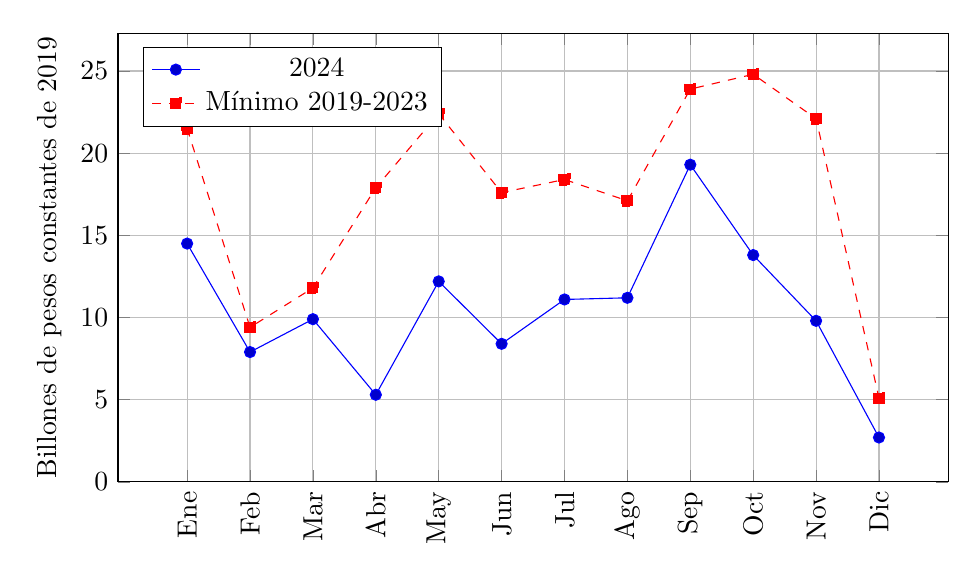
\begin{tikzpicture}
\begin{axis}[
    width=\textwidth,
    height=0.6\textwidth,
    ylabel={Billones de pesos constantes de 2019},
    xtick={1,2,3,4,5,6,7,8,9,10,11,12},
    xticklabels={Ene,Feb,Mar,Abr,May,Jun,Jul,Ago,Sep,Oct,Nov,Dic},
    xticklabel style={rotate=90, anchor=east},
    legend pos=north west,
    grid=both,
    ymin=0
]

% Valores de 2024
\addplot coordinates {
    (1,14.5) (2,7.9) (3,9.9) (4,5.3) (5,12.2) (6,8.4) 
    (7,11.1) (8,11.2) (9,19.3) (10,13.8) (11,9.8) (12,2.7)
};
\addlegendentry{2024}

% Mínimos de 2019 a 2023
\addplot[mark=square*, color=red, dashed] coordinates {
    (1,21.5) (2,9.4) (3,11.8) (4,17.9) (5,22.4) (6,17.6) 
    (7,18.4) (8,17.1) (9,23.9) (10,24.8) (11,22.1) (12,5.1)
};
\addlegendentry{Mínimo 2019-2023}

\end{axis}
\end{tikzpicture}
\vspace{0.1cm}
\par\footnotesize{\textit{Fuente: Elaboración propia con base en datos de la Dirección de Crédito Público, Ministerio de Hacienda.}}
\end{figure}
%\end{comment}

\begin{comment}
\begin{figure}
\centering
\caption{Depositos del Tesoro Nacional}\label{fig:depositos}
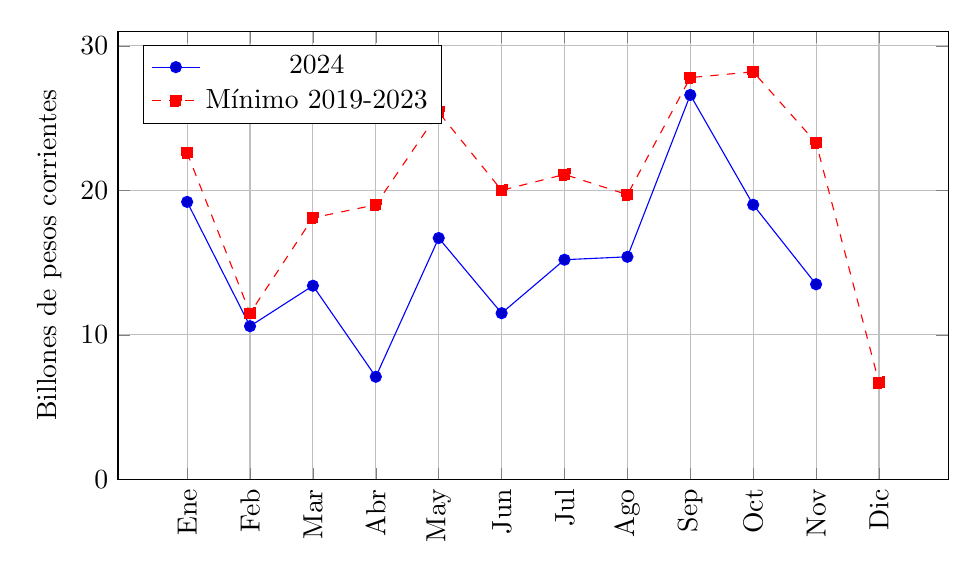
\begin{tikzpicture}
\begin{axis}[
    width=\textwidth,
    height=0.6\textwidth,
    %xlabel={Meses},
    ylabel={Billones de pesos corrientes},
    xtick={1,2,3,4,5,6,7,8,9,10,11,12},
    xticklabels={Ene,Feb,Mar,Abr,May,Jun,Jul,Ago,Sep,Oct,Nov,Dic},
    xticklabel style={rotate=90, anchor=east},
    legend pos=north west,
    grid=both,
    ymin=0
]

% Valores de 2024
\addplot coordinates {
    (1,19.2) (2,10.6) (3,13.4) (4,7.1) (5,16.7) (6,11.5) 
    (7,15.2) (8,15.4) (9,26.6) (10,19.0) (11,13.5) %(12,3.5)
};
\addlegendentry{2024}

% Media de 2019 a 2023
%\addplot coordinates {
%    (1,25.0) (2,21.6) (3,22.4) (4,26.5) (5,34.3) (6,31.6) 
%    (7,31.6) (8,29.2) (9,33.6) (10,31.4) (11,27.6) (12,10.6)
%};
%\addlegendentry{Media 2019-2023}

% Mínimos de 2019 a 2023
\addplot[mark=square*, color=red, dashed] coordinates {
    (1,22.6) (2,11.5) (3,18.1) (4,19.0) (5,25.4) (6,20.0) 
    (7,21.1) (8,19.7) (9,27.8) (10,28.2) (11,23.3) (12,6.7)
};
\addlegendentry{Mínimo 2019-2023}

\end{axis}
\end{tikzpicture}
\vspace{0.1cm}
\par\footnotesize{\textit{Fuente: Cálculos con base en datos de la Dirección de Crédito Público, Ministerio de Hacienda.}}
\end{figure}
\end{comment}

De hecho, los problemas de liquidez ya quedaron evidenciados a lo largo de 2024, como se observa en la Figura \ref{fig:depositos}. Esta muestra una pronunciada disminución en los depósitos del Tesoro Nacional en el Banco de la República, en comparación con los años 2019 a 2023. En ningún mes de 2024 los saldos superaron los registros del mismo mes en años anteriores. Dependiendo del acceso efectivo a financiamiento que logre el Gobierno tras la activación de la cláusula de escape, la disponibilidad de caja podría seguir actuando como una restricción de facto al gasto y al crecimiento del déficit. No obstante, esta forma de contención es solo un paliativo transitorio y no sustituye un ajuste estructural que corrija el desbalance fiscal de fondo.

En otras circunstancias, las dificultades de caja podrían haber llevado al Gobierno a considerar la financiación de su déficit a través de la emisión monetaria por parte del Banco de la República. Tal medida habría generado presiones inflacionarias que reducirían el poder adquisitivo de los colombianos. Afortunadamente, la Constitución garantiza la independencia del Banco, y cualquier préstamo al Gobierno requiere la unanimidad de su Junta Directiva. No obstante, la Junta no dejará de enfrentar presiones crecientes para reducir las tasas de interés. Por un lado, ceder a esta presión podría aliviar parcialmente el costo del financiamiento interno (aunque la incidencia de la tasa de política monetaria sobre la tasa de interés de la deuda pública de corto plazo parece ser cada vez más limitada). Por el otro, enviaría una señal de vacilación respecto al compromiso del Banco de la República con la estabilidad de precios y sugeriría que la política monetaria está siendo dominada por las necesidades fiscales. Esto a su vez generaría una expectativa de mayor inflación, que podría convertirse en una profecía autocumplida en la medida que hogares y empresas ajusten sus precios tratando de anticiparse a este evento.

En ausencia de respaldo monetario por parte del Banco de la República, el financiamiento del déficit fiscal recae principalmente sobre los compradores de títulos de deuda pública, como bancos comerciales, fondos de pensiones, aseguradoras, inversionistas extranjeros y organismos multilaterales. A diferencia de una regla fiscal estricta, este tipo de financiamiento no impone disciplina automática sobre las cuentas públicas. Por el contrario, algunos de estos inversionistas pueden seguir prestando incluso en contextos de deterioro fiscal, siempre que se les ofrezca una prima de riesgo suficientemente atractiva. Esta dinámica relaja las restricciones fiscales en el corto plazo, pero lo hace a costa de mayores tasas de interés, lo que encarece el servicio de la deuda y alimenta un círculo vicioso: el aumento del déficit conduce a mayor endeudamiento, y este, a su vez, incrementa el costo del financiamiento. Además, a medida que se deteriora el perfil fiscal del país, también cambia el perfil de sus acreedores: disminuye la participación de inversionistas institucionales conservadores con estrategias de largo plazo  y aumenta la de inversionistas con mayor apetito por el riesgo pero con horizontes de inversión más cortos. Esta transición incrementa la volatilidad de los mercados financieros y reduce la estabilidad del financiamiento público.

En este punto vale la pena retomar la discusión sobre el incumplimiento de la regla fiscal en 2024. ¿Qué hubiese pasado en 2025 si el Gobierno hubiese reconocido el incumplimiento de la regla fiscal en 2024? La \href{http://www.secretariasenado.gov.co/senado/basedoc/ley_1473_2011.html}{Ley 1473 de 2011} especifica que ``en cualquier caso de incumplimiento de la regla fiscal, el Gobierno Nacional deberá explicar detalladamente ... las razones del incumplimiento y fijar metas y objetivos tendientes a asegurar el cumplimiento de la misma.'' Al hacer lo que hizo el Gobierno en 2025 y desconocer inicialmente el incumplimiento de la regla fiscal en 2024, se pospuso la ejecución de medidas tendientes a retomar una senda sostenible para las finanzas públicas. La activación tardía de la cláusula de escape en junio de 2025 constituye, en los hechos, un reconocimiento parcial del desajuste acumulado.

Existe un debate legítimo sobre si las razones invocadas por el Gobierno para activar la cláusula de escape cumplen cabalmente con las causales previstas en la Ley 2155 de 2021. Más allá de esta discusión jurídica, lo que revela este episodio es una limitación más profunda del marco institucional colombiano: el país no cuenta hoy con instrumentos adecuados para enfrentar contingencias en las que la escasez de ingresos, combinada con un alto volumen de obligaciones legales de gasto, hace inviable el cumplimiento de la regla fiscal. En tales escenarios, el Gobierno se ve forzado a escoger entre violar el marco fiscal, incumplir obligaciones legales o recurrir a mecanismos extraordinarios como la cláusula de escape. Como se analiza en el Capítulo \ref{chap:normas}, se requieren reformas institucionales que permitan manejar de manera más ordenada y previsible este tipo de tensiones sin recurrir a la cláusula de escape.

La activación de la cláusula de escape obliga ahora al Gobierno a establecer una ``senda de retorno al pleno cumplimiento de las metas fiscales''. Sin embargo, diseñar e implementar una senda creíble requiere no solo voluntad política, sino también la búsqueda de consensos que permitan viabilizar las reformas legales necesarias para el ajuste fiscal. Desafortunadamente, 2026 es un año electoral, lo que hace prever que las decisiones de consolidación fiscal más difíciles serán postergadas y que el diseño y la implementación efectiva del plan recaerán principalmente en la próxima administración. Este retraso incrementa el riesgo de que la cláusula de escape se perciba como una licencia para dilatar los ajustes necesarios, lo que podría erosionar aún más la credibilidad de la regla fiscal y complicar el acceso a financiamiento en los mercados.

%En cualquier caso, ante la activación de la cláusula de escape, sólo la disponibilidad de caja limitará el gasto efectivo que se realice en 2025, condicionando el monto del déficit fiscal. Esta escasez de efectivo y no la regla fiscal será la que determine el balance fiscal al finalizar el año. Mientras tanto, se tendrá que definir a través del manejo de caja qué gastos se priorizarán y cuáles se aplazarán en la forma de compromisos que se trasladarán al año siguiente.

Más allá de los desafíos inmediatos que se presentan en 2025, el saneamiento de las finanzas públicas necesariamente tiene que pasar por soluciones estructurales que tomarán tiempo en hacerse efectivas, pero que deben diseñarse, discutirse y legislarse lo más pronto posible. La discusión de estas soluciones debe comenzar desde ya, dada la peligrosa dinámica que está adquiriendo la deuda pública, como se discute en el Capítulo \ref{chap:perspectivas}.
